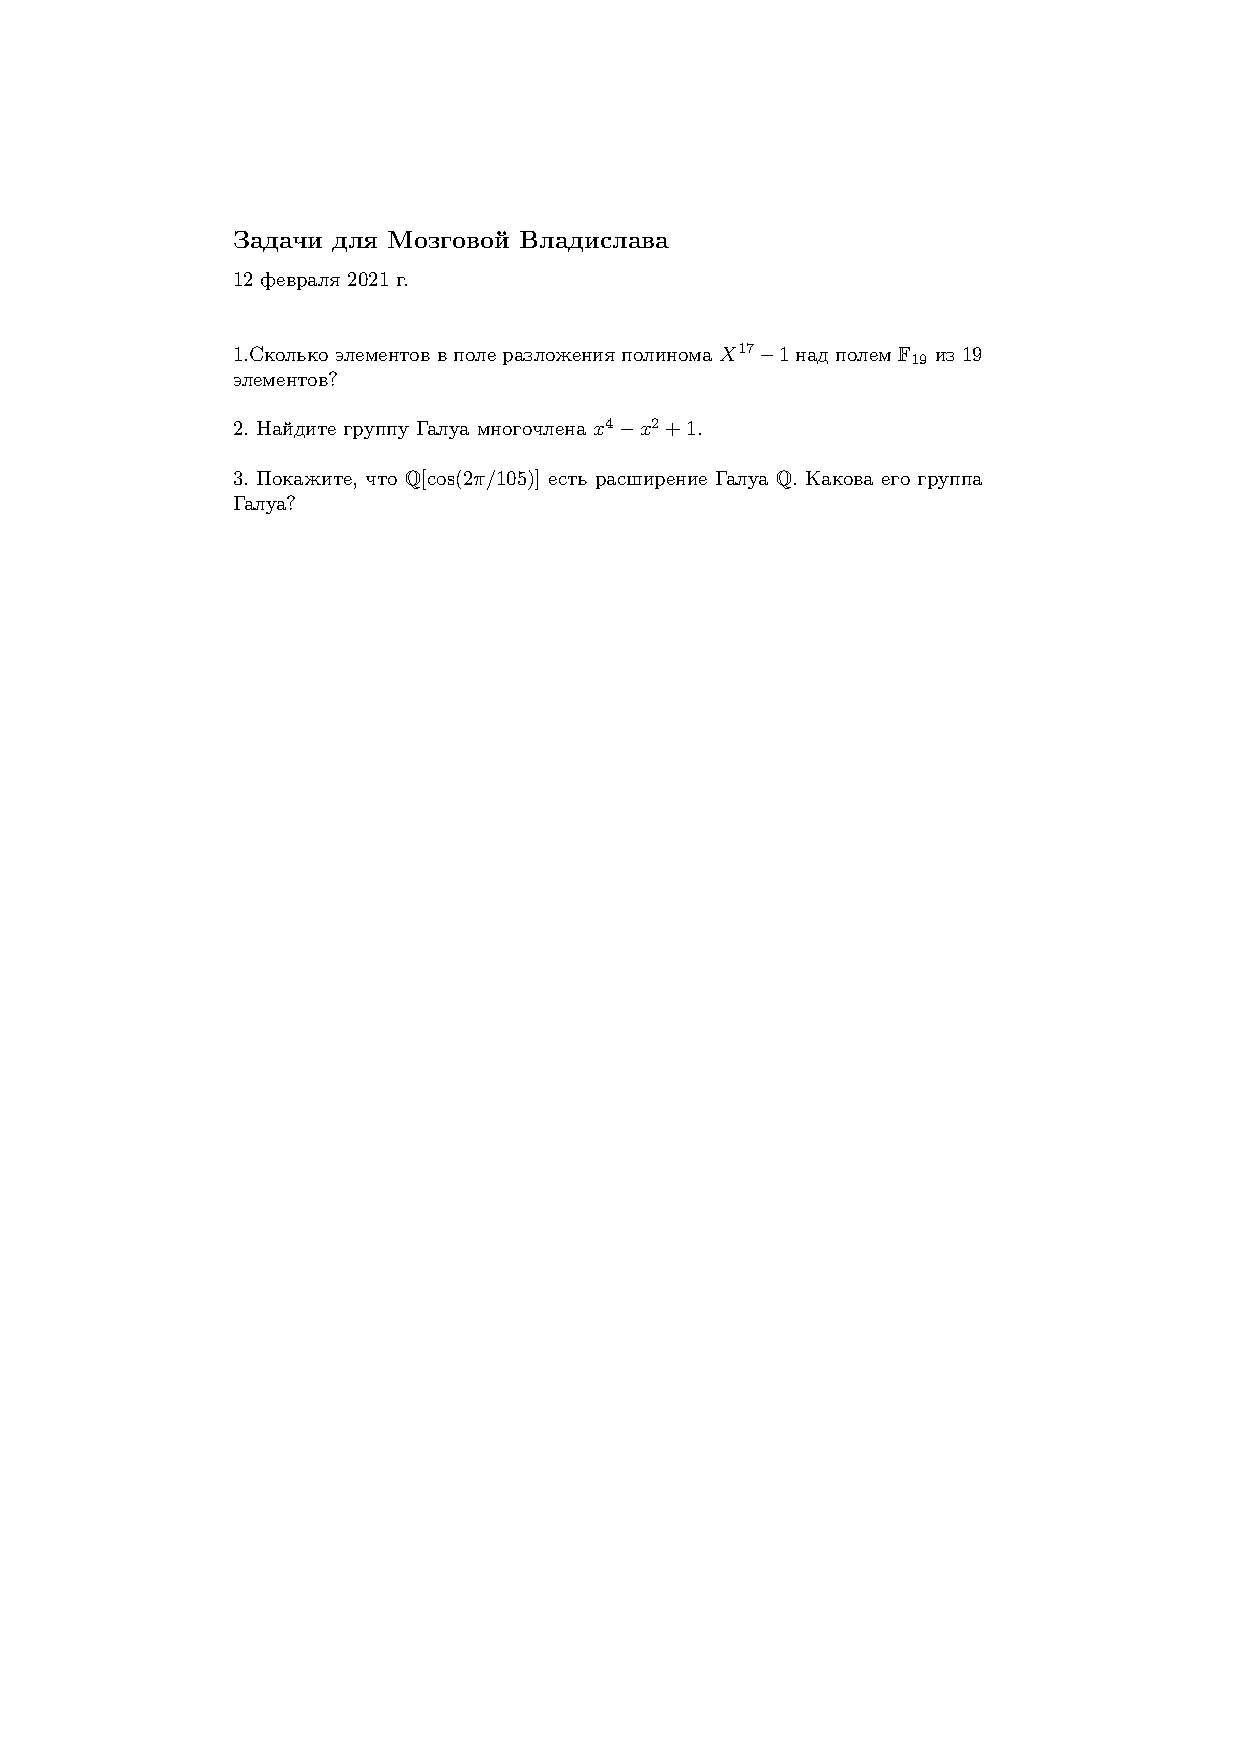
\includepdf[scale=1,pages=1]{Tasks/problem.pdf}
\newpage
\section*{Решения}
\subsection*{Задача 1}
	$x^{17} - 1 = (x-1) \Phi_{17}$. $\forall x \in \mathbb{F}_{19}\ x^18 = 1,\ x \ne 0$. Всякое расширение $\mathbb{19}$ имеет вид $\mathbb{F}_q\ (x^{q-1} = 1),\ q = (19)^f$ так как $\mathbb{F}_q$ -- векторное пространство над $\mathbb{F}_{19}$. Рассмотрим $\mathbb{F}_{q}* = \mathbb{Z}_{(q-1)}$, мы хотим чтобы там был элемент порядка $17$. Что такое поле разложения над конечным полем? -- мы можем взять $\mathbb{F}_19$ и присоединить алгебраические корни. Рассмотрим все конечные поля $(19)^f$, они упорядочены. Поле разложения -- наименьшее из полей, содержащее все корни уравнения, тогда
	\begin{gather*}
		19^f \equiv 1 \mod 17\\
		f = 8
	\end{gather*}
	Ответ: 8
\vskip 0.4in

\subsection*{Задача 2}
	\begin{gather*}
		x^4 - x^2 + 1\\
		f(x) = x^4 + a_3x^3 + a_2x^2 + a_1x + a_0\\
		a_0 = 1,\ a_1 = 0,\ a_2 = -1,\ a_3 = 0
	\end{gather*}
	Кубическая резольвента имеет вид
	\begin{gather*}
		g(x) = x^3 + b_2 x^2 + b_1 x + b_0\\
		b_2 = -a_2 = 1\\
		b_1 = a_1 a_3 - 4a_0 = 0 \cdot 0 - 4 \cdot 1 = -4\\
		b_0 = 4a_0 a_2 - a_1^2 - a_0 a_3^2 = 4 \cdot 1 \cdot (-1) - 0^2 - 1 \cdot 0^2 = -4\\
		g(x) = x^3 + x^2 - 4x - 4 = (x+1)(x-2)(x+2)
	\end{gather*}
	Проверим, является ли дискриминант полным квадратом
	\begin{gather*}
	\begin{vmatrix}
		1 & 0 & -1 & 0 & 1 & 0 & 0\\
		0 & 1 & 0 & -1 & 0 & 1 & 0\\
		0 & 0 & 1 & 0 & -1 & 0 & 1\\
		4 & 0 & -2 & 0 & 0 & 0 & 0\\
		0 & 4 & 0 & -2 & 0 & 0 & 0\\
		0 & 0 & 4 & 0 & -2 & 0 & 0\\
		0 & 0 & 0 & 4 & 0 & -2 & 0
	\end{vmatrix}
	= 144 = 12^2
	\end{gather*}
	Следовательно группа Галуа $V_4$

\begin{comment}
	$x^4 - x^2 + 1$, пусть $a = x^2$, тогда $a^2 - a + 1 = 0$, $a_1 = \frac{1 + i\sqrt{3}}{2},\ a_2 = \frac{1 - i\sqrt{3}}{2}$, откуда корни начального это $x_1 = \frac{i + \sqrt{3}}{2},\ x_2 = \frac{i - \sqrt{3}}{2},\ x_3 = \frac{-i + \sqrt{3}}{2},\ x_4 = \frac{-i - \sqrt{3}}{2}$. Присоединим $\sqrt{3}$ и рассмотрим $\mathbb{Q}[\frac{i\sqrt{3}}{2}]$, $(1 - i\sqrt{3})(1 + i\sqrt{3}) = 4$. Если в поле есть $\sqrt{\frac{1 - i\sqrt{3}}{2}} = \frac{i + \sqrt{3}}{2}$ (или просто $i + \sqrt{3}$), то есть и все остальные корни.
	\begin{gather*}
		\frac{i + \sqrt{3}}{i} = -i(i + \sqrt{3}) = 1 - i\sqrt{3}\\
		\mathbb{Q}[i\sqrt{3}, 1 - i\sqrt{3}] \text{ -- поле расширения}
	\end{gather*}
	Минимальный многочлен $i\sqrt{3}$ это $f_1 = x^2 + 3 = 0,\ \deg f_1 = 2$, минимальный многочлен $1 - i\sqrt{3}$ это $x^2 + 2i\sqrt{3} + 2$\\
	$\deg L|_{Q} = 4$ и группа Галуа $\mathbb{Z}_2 \times \mathbb{Z}_2 = V_4$
\end{comment}
\vskip 0.4in

\subsection*{Задача 3}
	$\cos \frac{2\pi}{105} = \frac{\omega + \omega^{-1}}{2}$, где $\omega$ -- корень из 1. $K = \mathbb{Q}(\omega),\ \varphi \in \operatorname{Gal}(K|Q)$ -- автоморфизм $K|Q$, такой что $\omega \to \omega^{-1}$.\\
	$\operatorname{Aut}_{\mathbb{Q}}K|Q$ оставляет на месте $\mathbb{Q}$ и не оставляет $K|Q$. $K|Q$ получен из $\mathbb{Q}$ добавлением $\omega$, а следовательно автоморфизм определен тем, куда переходит $\omega$. $\omega \to \omega^{-1},\ \omega^{-1} \to \omega,\ \omega + \omega^{-1} \to \omega + \omega^{-1} \in$ подполе инвариантов.\\
	$\varphi^{2} = \operatorname{id}$, откуда $\langle \varphi \rangle = \mathbb{Z}_2$. $L = \mathbb{Q}(\cos \frac{2\pi}{105}),\ L = K^{\langle \varphi \rangle} = K^{\varphi} \subset K$. о основной теореме теории Галуа $\operatorname{Gal}(L|Q) = \operatorname{Gal}(K|Q)|_{\langle \varphi \rangle}$. ледовательно нужно посчитать $\operatorname{Gal}(K|Q) = (\mathbb{Z}_{105})*$ и профакторизовать по $\mathbb{Z}_{2}$\\
	$|\operatorname{Gal}(K|Q)| = \varphi(105) = 48$, откуда порядок $\operatorname{Gal}(K|Q)|_{\langle \varphi \rangle}$ -- $\frac{48}{2} = 24$. $(\mathbb{Z}_{175})* = (\mathbb{Z}_{3})* \times (\mathbb{Z}_{5})* \times (\mathbb{Z}_{7})* = \mathbb{Z}_{2} \times \mathbb{Z}_{4} \times \mathbb{Z}_{6} = \mathbb{Z}_{2} \times \mathbb{Z}_{2} \times \mathbb{Z}_{3} \times \mathbb{Z}_{4}$. Откуда $\mathbb{Z}_{3} \otimes \mathbb{Z}_{4} = \mathbb{Z}_{12}$.
\begin{comment}
	Заметим, что $\cos \frac{2\pi}{105} = \frac{e^{\frac{2\pi i}{105}} + e^{-\frac{2\pi i}{105}}}{2}$ и $\mathbb{Q}[e^{\frac{2\pi i}{105}}] = \mathbb{Q}[\sqrt[105]{1}]$. По теореме из лекции $\deg L_{105}|_{\mathbb{Q}} = \varphi(105) = 48$ и $\operatorname{Gal} L_{105}|_{\mathbb{Q}} \simeq (\mathbb{Z}_{105})* \simeq (\mathbb{Z}_{3})* \times (\mathbb{Z}_{5})* \times (\mathbb{Z}_{7})* = \mathbb{Z}_{2} \times \mathbb{Z}_{4} \times \mathbb{Z}_{6} = \mathbb{Z}_{2} \times \mathbb{Z}_{2} \times \mathbb{Z}_{3} \times \mathbb{Z}_{4}$\\
	$\deg(\mathbb{Q}[\cos(e^{\frac{2\pi i}{105}})]|_{\mathbb{Q}}) = 4$, цикл расширрения степени 4. $\cos(e^{\frac{2\pi i}{105}})$ -- корень уравнения $x^2 - 2\cos(\frac{2\pi}{105})x + 1 = 0$, откуда $x = \frac{2\cos(\alpha) \pm 2i\sin(\alpha)}{2} = \cos(\alpha) \pm i \sin(\alpha)$, степень расширения 2, откуда $\deg(\mathbb{Q}(\cos(\frac{2\pi}{105}))|_{\mathbb{Q}}) = 2$, по основной теореме Галуа $\mathbb{Q}(\cos(\frac{2\pi}{105}))$ -- расширение Галуа и группа $\mathbb{Z}_2$
\end{comment}